\documentclass[twocolumn,letterpaper,10pt]{article}
%\usepackage[T1]{fontenc}
\usepackage{amsmath}
\usepackage{listings}
\usepackage{booktabs}
\usepackage{url}
% The following is needed in order to make the code compatible
% with both latex/dvips and pdflatex.
\ifx\pdftexversion\undefined
\usepackage[dvips]{graphicx}
\else
\usepackage{graphicx}
\DeclareGraphicsRule{*}{mps}{*}{}
\fi

\newcommand{\naive}{na\"{\i}ve }


\title{CSEE4824 Course Project}
\author{Danqing Hua $<dh2604@columbia.edu>$\\
  Jiacheng Yang $<jy2522@columbia.edu>$}
\date{December 2012}

\begin{document}

\maketitle

\section{Introduction}
\label{sec:intro}

In this report, we describe our work towards the course project in
CSEE4824 Computer Architecture 2012 Fall. In this project, we are asked to optimize for a specific matrix
operation workload and to design a computer architecture for this
workload.

We focus our optimization on standard matrix multiplication
algorithm. We aim to optimize our code in an architecture-sensitive
way, such that we fully exploit the ILP and TLP in hardware. We also discuss
several optimizations, which do not work on
our hardware configuration, such as cache blocking, and justify the reason.

We start our architecture configuration from a single-core architecture. Based on that, we find
another multi-core design and compare these two options.

Our report is structured as follows. In Section ~\ref{sec:software}, we introduce our software optimization
techniques to exploit instruction-level parallelism and
thread-level parallelism. In Section ~\ref{sec:design}, we introduce how to explore the
design space in a systematic way. We show our experimental results on
both software optimization and architecture tuning in Section
~\ref{sec:exp}. We conclude our report in Section ~\ref{sec:conclude}.

\section{Software Optimization}
\label{sec:software}

Among the four matrix operations, we focus on optimizing matrix
multiplication, because it has the highest computational complexity
$O(n^3)$. Amdahl's law suggests that we should improve the dominant
operation to achieve a significant overall speed-up.

Standard matrix multiplication has $O(n^3)$ complexity. Strassen
algorithm~\cite{CLRS} is a well-known algorithm which has a lower
complexity of $O(n^{2.81})$. However, Strassen algorithm is not applicable to our problem. First, the test
case is not big enough to cover the constant factor in Strassen
algorithm. The biggest test case is of size 201, $201^3 = 2.73 *
201^{2.81}$. In order to make Strassen algorithm faster, the
constant cannot be more than 2.73. The additional work
to apply the Strassen algorithm, e.g. padding the matrix with 0, malloc
temporary matrix and recursive function call is overwhelming. Second, Strassen is not
easy to parallelize. Thread spawning are required in a child thread,
which is not supported by $SESC$.

So we focus on optimizing standard matrix
multiplication algorithm, but in an architecture-sensitive way. We will introduce the techniques to
optimize the other three operations as well at the end of this
section.

\subsection{Loop Ordering}
First of all, for matrix multiplication, there are mutliple ways to order the
loops. We choose the i,j,k ordering in our implementation, because
we are able to use a register to store the temporary result
$r(i,j)$. Other ordering may enable us to reference elements in input
matrix A or B by register. However, in general memory write is more
costly than memory read, so it's better for us to buffer the
write into a register. Within this ordering, we also benefit from
spatial locality in both input matrices after we transpose matrix $B$.

\subsection{Transpose Matrix B}
In the original matrix multiplication, the data access to matrix $B$
in the inner loop is not sequential. It reads $B$ with a stride length
of $n$. If no optimization is made, it will
introduce more cache misses, even TLB misses. To alleviate such
overhead, we transpose the matrix $B$ in advance, so that the access pattern
to matrix $B$ in the inner-loop is sequential. As we will show later,
we benefit from a large cache-line, especially when all reads are sequential.

\subsection{Loop Unrolling and Register Reusing}
Since we are not allowed to use any compiler optimization, we have to
do loop unrolling ourselves. Loop unrolling has at least the following
two advantages: (1) reduce branches (2) use registers to avoid memory
access. By loading a common value used in an outer-loop in a register,
we avoid fetch the data repeatedly from L1 or L2 caches~\cite{revisited,berkeley}. Combining
loop unrolling and register reusing gives us high performance gain.

In our implementation, we have two layers of loop unrollings. The first
is unrolling the inner-loop (indexed by $k$). The main purpose of this
unrolling is to reduce branches and increase ILP.

We also unroll the outer-loop (indexed by $j$). Because
the inner-loop is tight, we still have abundant available
registers. If we use registers as another memory hierarchy~\cite{revisited},
we can further speed up our program. Meanwhile, although the access to
$a(i,k)$ in the inner-loop is not replaced by a register, since we
organized the code in a compact way, the value of $a(i,k)$ is likely
to be kept in a register, so a large number of memory traffic is
saved. Our experiment shows that these two techniques altogether
speedup the overall performance by 1.5.

\subsection{Cache Blocking}
Cache blokcing is a technique to improve cache behavior of matrix
multiplication~\cite{block}. Basically, it breaks down the matrix into smaller
blocks that can be held in L1/L2 cache. It uses a block as much as
possible after loading it from memory. The ideal block size is
the maximum block size that can hold the entire blocks in L1 cache. It
is calculated as~\cite{davis},
\begin{equation}
  2 * BlockSize^2 * wordSize = L1\ Cache\ Size
\end{equation}

If we use a 16K L1 cache, the block size is 32. Additionally, we also like the block
size to be a multiple of the cache-line size.

We implemented the cache blocking algorithm, but the experiment shows
us that the saving effect of cache blocking is not significant in our
configured system. Instead, it performs even worse than non-blocking
algorithm, even if the simulation result shows a much lower L1 miss rate.

The reason for this degradation is that the miss penalty of L1/L2 miss
is too small. Even if we apply a huge L2 cache with 1M cache size, the
access time to this cache is only 2-3 cycles. Meanwhile, such a small miss
penalty is very likely to be hidden by instruction-level
parallelism. When an instruction is stalled waiting for data from L2
cache, other instructions will continue executing, keeping the CPU busy.

In addition, cache blocking actually counteract with the advantage of
register reusing. If a matrix is partitioned into four parts, then
each element in the resulting matrix needs to be written fourth. When 
there is no cache blocking, we only need to write each element
once because other update to that element is done in the register.

We verify our idea by increasing the access time of L2 cache (instead
of using the given formula). Our experiment shows that with the
increased L2 access time, cache blocking becomes more important (see
Section ~\ref{sec:exp}).

\subsection{Multi-threading}
We use multi-threading to achieve thread-level parallelism
. The workload in this project is a perfect fit for multi-threading because
the work can be evenly partitioned, so there is no skewness. And the
work can be processed independently, so there is no contention. In addition, we will benefit from the potential power efficiency of
multi-core architecture.

There are various ways to parallelize the execution of matrix
multiplication. In our implementation, we simply partition the rows of
the output matrix. Each thread works to compute the rows
that are assigned to it. We partition the work in this way because
these works are independent, so race condition does not
exist. Considering the implementation of $SESC$'s threading library, we
highly doubt the efficiency of its mutex/locking implementation.

Our experiment in Section ~\ref{sec:exp} verifies that our multi-threading implementation brings
us a nearly-linear speed-up.

\subsection{Optimizing other operations}
We also optimize for the remaining three operations: scaling, addition
and vector multiplication. 

The technique we used to optimize these operations are mainly
multi-threading and loop-unrolling. We partition the work by rows similarly as
in matrix multiplication. Loop unrolling is used to reduce branch misprediction.

The access pattern of these three operations are quite simple. For
scaling and addition, each element is read only once, so there is no
temporal locality here. But we can benefit from spatial locality if we
read the data sequentially. That leads us to a larger cache-line size.

For matrix-vector multiplication, the matrix is read once, while the
vector is read multiple times. Although we can also use cache blocking
to improve the cache behavior of the vector, we find it not necessary
in this workload. The vector in the large test case is only
201. Suppose one cache line is left for the matrix, and one cache line
is left for the output vector. Our L1 cache is big enough to hold the
entire vector. Thus, we do not optimize specifically for the cache
behavior of matrix-vector multiplication.


\section{Exploring the Design Space}
\label{sec:design}

The general principle of our exploration is that we start from simple
parameters. We gradually fix more parameter and tune for an unknown parameter. Lessons from the
architecture course greatly helps us reduce the search space.

\subsection{Single-core}
We start exploring the design space from a single-core design. Let's
first assume that we've figured out the best cache configuration. We
will talk about how we choose cache next. In general, we first use
small and medium test case to find reasonable candidate designs
conforming to the power constraint before we run simulation on large test case.

\paragraph{Inorder v.s Out-of-order:} Our intuition is that
out-of-order is much better than inoder execution because of ILP. We
verify this by the following micro-benchmark on a large test case.

The result clearly demonstrates the advantage of out-of-order
execution over in-order execution, even if the issue width of the
out-of-order execution is only 1.

\begin{table}[ht!]
\begin{center}
\begin{tabular}{ccccc}
\toprule
Execution   &  Freq  & Issue width  &  time  & power \\
\midrule
In-order   &  1G  &  1  &  2527  &  4.6 \\
Out-order     &  1G &  1  &    594 & 14.3 \\
\bottomrule
\end{tabular}
\end{center}
\caption{Comparing in-order and out-of-order}
\end{table}

The power of out-of-order execution is much higher than in-order execution. In-order execution
consumes less power because most of its time is spent on stall. From
the detailed power consumption, we can tell that a
large part of its power is spent on clock instead of on execution. So using in-order execution
actually wastes more power. Thus, we adhere our following exploration to out-of-order execution.

\paragraph{Issue width:} Issue width influences the instruction-level
parallelism we can achieve. On MidCore and LargeCore, higher issue width also means
more functional units. So we suggests that the larger is the issue width,
the better the performance is.

On an moderate size test case, we fix all other parameters and vary the issue
width. The result in Figure ~\ref{fig:issue} shows that as the issue width
increases, the execution time decreases. But after issue width
increases over 4, the execution time stops improving on all types of cores. We conclude that the
instruction-level parallelism is fully exploited in such cases. Continuing
increasing issue width will only increase the cost of maintenance, such as the access time to the re-order buffers.

\begin{figure}[ht!]
\begin{center}
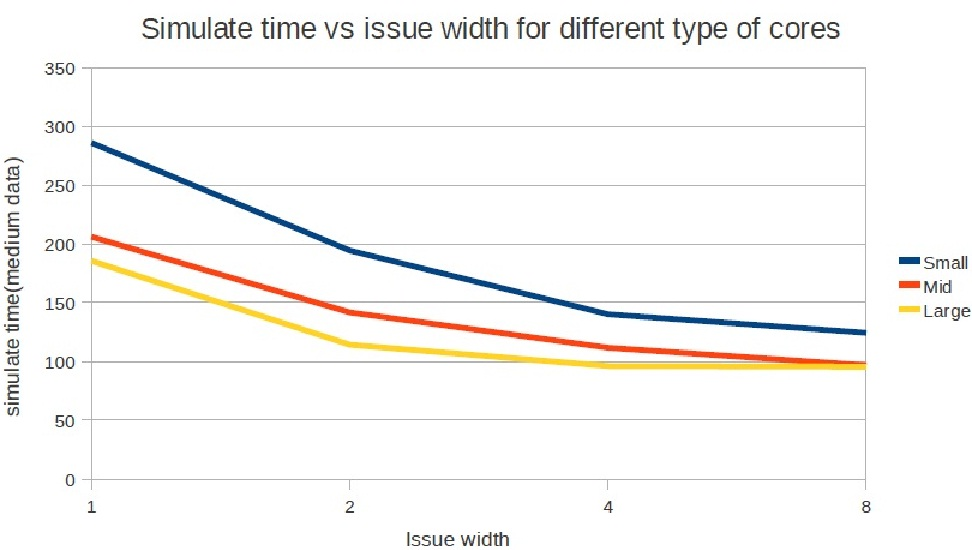
\includegraphics[width=0.4\textwidth]{figures/issue.jpg}
\end{center}
\label{fig:issue}
\caption{Simulation time V.S issue width}
\end{figure}

\paragraph{Type of cores:} Each type of core varies by their number of
execution units and ROB size. At a first glance, large core may be the
first choice, as it carries more powerful functional units. However,
we also have to lower the frequency to meet the power
constraint. There is no clear good or bad in choosing the type of
cores. Each core combining with appropriate issue width and frequency
may meet the power constraint while preserve a good performance. But some
preliminary experiments let us prefer SmallCore and MidCore because
they usually have a competitive performance within a reasonable power budget. 

We dismiss the idea for a heterogeneous multi-core architecture in
this project, because the workload is partitioned into equal size. It
doesn't make sense to bias one thread or another by giving it a more
powerful core.

\paragraph{Frequencies:} The guideline for tuning frequency is: as
high as possible within the power constraint. So we usually tune the
frequency after all other parameters are fixed.


\subsection{Multi-core}
Exploring the design space of single-core design provides us useful
hint to explore multi-core designs. Our experiment in Section ~\ref{sec:exp} shows
that our program has a linear speed-up. So introducing more
cores, presumably is better. But considering the power constraint, we
focus on a dual-core architecture to illustrate what is new in
a multi-core architecture.

An interesting observation from the multi-core design is the power
efficiency of multi-core architecture. We measure the power efficiency of an architecture as performance per
Watts. Performance is measured by KIPS (kilo-instructions-per-second)
from $SESC$'s result. We plot the power efficiency of architectures
with different number of cores. We can see in Figure ~\ref{fig:power} that as the number of cores
increases, the power efficiency also increases.

\begin{figure}[ht!]
\begin{center}
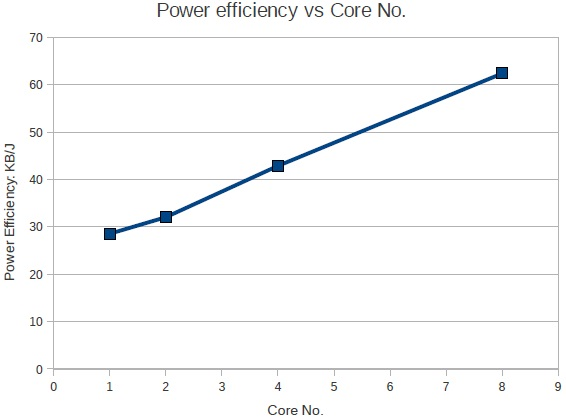
\includegraphics[width=0.4\textwidth]{figures/efficiency.jpg}
\end{center}
\caption{Power efficiency V.S number of cores}
\label{fig:power}
\end{figure}

\subsection{Configuring Cache}

\subsection{Cache Hierarchy}
For single core architecture, a two-level cache hierarchy is a better
choice. L1 cache guarantees fast access, while the larger L2 cache stores
more data to avoid the penalty of memory access.

For multi-core architecture, we prefer a shared-L2 hierarchy. 
In our workload, matrix $B$ is shared by all
threads. Using a private L2 cache will only lead to unnecessary cold
start.  

\subsubsection{L1 Cache}
Our code is very small, so we don't need a large L1 instruction
cache. We fix L1 instruction cache to its minimum size 16K. L1 data
cache is chosen to 16K as well, mainly because it saves power and L2
cache access is cheap in this project.

\subsubsection{L2 Cache}
Unlike L1 cache, whose size has a significant influence on
power. Enlarging L2 cache seems to come for free. We vary the size of
L2 cache from 128K to 1M, the power remains stable, and the access
time is within 3 cycles if we set the associativity to 8 and banks to
2. The total size of three matrices is $201 * 201 * 3 * 8 = 946K$, so
a 1M L2 cache can hold every data. Misses in L2 cache in this case are
due to compulsory misses during matrix generation or contention
misses.

\subsubsection{Cache block size}
Because almost all reads are sequential in this workload, we want to
use a larger block size. We set the block size to 64
bytes, because it guarantees a low access to L1 cache and it won't
bring in too much unnecessary data at the boundary of a row or a partition.

\section{Experiment}
\label{sec:exp}
In this section, we illustrate some experimental results to support
our claims in Section ~\ref{sec:software} and Section ~\ref{sec:design}.
 
\subsection{Cache Blocking}
We mentioned in Section ~\ref{sec:software} that cache blocking does not give us
too much performance gain. Instead, it hurts our performance.

First, we show the result by varying block size in one of our best
single-core configurations: 1.8 GHz MidCore, issue width = 2. The L1
cache is 16KB, and the L2 cache is 1M, block size is 64 bytes. The workload is medium. We also
measures the execution time of matrix generation, which is roughly 1.9
msec. After subtracting this start-up time from the result, the trend
becomes more clear. Note that the L1 cache is smaller than the two input
matrices.

Here, we find the following observations (1) the best block size is
smaller the ideal block size we calculated before (2) in our workload,
the performance downgrades with blocking. The best block size should be smaller because
the L1 cache may also contain some other data. And if we take a look
at the matrix size, we find that 71=24*3-1, however 71=32*3-25. So
when the block size is 32, actually most work in the last pass is
wasted. Note that 24 is also multiple of the cache-line size, which is
64 bytes, or 8 elements.

\begin{table}[ht!]
\begin{center}
\begin{tabular}{ccccc}
\toprule
Block size & Time & L1 miss & L2 miss & DRAM access \\
\midrule
16 & 6.944 & 0.67\%	 & 12.21\%	& 0.53\% \\
24 & 6.682 &  1.01\% &	8.54\%	& 0.80\% \\ 
32 & 6.711 & 1.66\%	 & 5.19\%	& 1.31\% \\ 
40 & 6.585 &  1.89\% & 4.70\%	& 1.48\% \\ 
no blocking	& 6.514	& 1.78\% & 5.08\%	& 1.40\% \\
\bottomrule
\end{tabular}
\end{center}
\label{fig:blocking}
\caption{Cache blocking: Effect of block size}
\end{table}


To see how the cache blocking algorithm takes effect, we increase the
access time of L2 cache. The result is shown below. It is interesting
to see that when the gap between L1 cache and L2 cache increases, 
cache blocking becomes more important. To make it one step further,
blocking will have more effect in reducing L2 cache miss. Since the
gap between L2 and memory is usually even larger, hundreds of cycles,
it is likely to improve the performance greatly. However, in our
workload, the largest test case can almost be fit in the L2
cache. Thus, we cannot see such performance gain.

\begin{table}[ht!]
\begin{center}
\begin{tabular}{cccc}
\toprule
L2 access time & Ideal	& Nonblocking & speedup\\
\midrule
3 &	6.682 & 6.514 & 0.97 \\ 
30 & 6.899  & 7.168 & 1.04 \\ 
50	& 7.082	& 8.036 & 1.13  \\ 
100	& 7.589	& 10.647 & 1.40 \\ 
200	& 8.624	& 15.888 & 1.84\\
\bottomrule
\end{tabular}
\end{center}
\caption{Cache blocking: Effect of L2 access time}
\end{table}


\subsection{Loop Unrolling}

Not let's look at the effect of loop unrolling and how we choose the
best number of unrollings we made based on our experiment. It is clear
from the result that unrolling the $j$ loop 3 times is the best
choice. We always unrolling the inner-most loop for 4 times for
simplicity. But you can change it to 2 by a switch in the code.

\begin{table}[ht!]
\begin{center}
\begin{tabular}{ccccc}
\toprule
Unrolling & time & L1 miss  & L2 miss & Speedup \\
\midrule
No unrolling & 10.211 & 1.93 & 5.04	& 1.3 \\
Rolling 2 & 6.821 & 1.81 & 5.08 & 1.38 \\
Rolling 3 & 6.515 & 1.78 & 5.08 & 1.4 \\
Rolling 4 &	6.59 & 1.64	& 5.08 & 1.42 \\
\bottomrule
\end{tabular}
\end{center}
\caption{Speedup of loop-unrolling}
\label{fig:unrolling}
\end{table}


\subsection{Multi-threading}

We test the scalability of our multi-threading program. In this
experiment, we ignore the power constraint: we just assign more cores
and study the speedup. Again, we are doing experiment on the medium
test case, but all time we report below is the time subtracting the
program start-up time (matrix generation, etc). Our basic
configuration is $n$ MidCore with issue width 2, we vary $n$. Each core
has 16K L1 Instruction cache and 32K L1 Data cache. The L2 shared
cache is 256K. We use out-of-order execution and set the frequency to 1.8GHz.

The following figure shows the scalability of our algorithm. When we
scale the number of threads from 1 to four, it has almost a linear
scale-up. When the number of threads reaches 8, we have a sub-linear
scale-up. Although there is no contention here, adding more threads will
saturate the memory bus, and the coordination cost increase. And the
execution is dominated by the slowest thread. So we cannot have linear
scale-up with too many threads.

\begin{figure}[ht!]
\centering
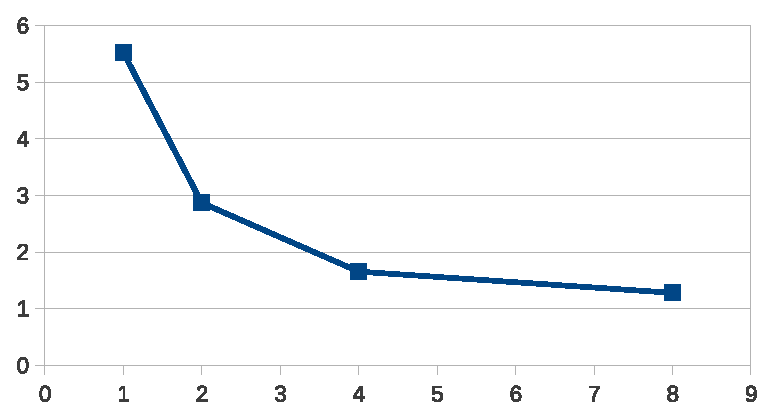
\includegraphics[width=0.4\textwidth]{figures/scale2.eps}
\caption{Scaling with more threads}
\end{figure}

(What need to mention is that, during our development, we decompose
each operation and test its scalability separately)

\subsection{Final Performance}
We report the final performance of our architecture and program. We
give two configurations here, one for single-core architecture and the
other for multi-core architecture. The config file we submit at last
is the multi-core version. Our configurations for both architectures
are shown in Table ~\ref{table:config}.

\begin{table}[ht!]
\begin{center}
\begin{tabular}{ccccc}
\toprule
& Single & Multi \\
\midrule
Core type & Mid & Small \\
Inorder & false & false \\
Issue width & 2 & 2 \\
Frequency & 2.1G & 1.6G \\
Cache Org & L2Single & L2Share \\
L1 Cache & 16K & 16K \\
L2 Cache & 512K & 256K \\
Block size & 64 & 64 \\
\bottomrule
\end{tabular}
\end{center}
\caption{Configurations for Single-core and Multi-core architecture}
\label{table:config}
\end{table}

For single-core architecture, the performance on three test cases are
reported in Table ~\ref{table:single}.

\begin{table}[ht!]
\begin{center}
\begin{tabular}{ccccc}
\toprule
Test  & time & L1 miss(\%)  & L2 miss(\%) & Power \\
\midrule
Small & 0.606 & 0.29 & 56.76& 25.131 \\
Medium  & 5.585 & 1.78 & 5.08 & 27.907 \\
Large & 100.055 & 1.89 & 5.97 & 29.493 \\
\bottomrule
\end{tabular}
\end{center}
\caption{Single-core final result}
\label{table:single}
\end{table}


Multi-core architecture's result is shown in Table ~\ref{table:multi}.
\begin{table}[ht!]
\begin{center}
\begin{tabular}{ccccc}
\toprule
Test  & time & L1 miss(\%)  & L2 miss(\%) & Power \\
\midrule
Small &  0.725 & 0.28 & 65.21 & 22.447 \\
Medium  & 5.9 & 1.6 & 9.77 & 27.505 \\
Large  & 103.247 & 1.64 & 95.82  & 29.848 \\
\bottomrule
\end{tabular}
\end{center}
\caption{Multi-core final result}
\label{table:multi}
\end{table}

From the result we can see that there is no clear winner between a
single-core and multi-core design. In this application, there is
abundant instruction-level parallelism: instructions and data are
mostly independent, data dependency is less. With software
optimization, such as loop-unrolling, we can exploit ILP to the
extreme. Single-core architecture is also more simple and
efficient. We tried to use `L2Shared' model with one thread, and it performs
much worse than the `SingleL2' model. Although our multi-core architecture does not win over the single-core
design within this power constraint, by our experiment, we show that
our algorithm design is scalable with the number of cores.

\section{Conclusion}
\label{sec:conclude}

In this report, we summarize our techniques to optimize matrix
operations for the given workload. We use pre-processing, software loop-unrolling,
register reusing to enhance the execution of single thread
execution. We investigate cache-aware matrix multiplication and their
impact on our system's performance. We apply multi-threading to
parallelize all the operations and we experimentally show that we
achieve a nearly-linear scale-up when the number of cores is less than 8.

We systematically explore the design space, finding out the best
architecture for both uni-core architecture and dual-core
architecture. Instead of enumerating all possibilities in the design
space, our search is guided by our understanding in architecture
concept, so we greatly reduce the search space.

Finally, we experimentally verify our design and quantify the speedup
in our software optimization.

\bibliographystyle{plain}
\bibliography{refs}

\end{document}
